\section{Results and Discussion}

\subsection{Performance Comparison Across Configurations}
Table~\ref{tab:main_results} reports the best case per bank based on mean RMSE across five seeds. BiLSTM-based settings are dominant in six out of seven banks. The best configurations are mostly \texttt{bilstm\_without\_macro}, with two bank-specific exceptions: \texttt{bilstm\_without\_macro\_ga} for BBTN and \texttt{bilstm\_with\_macro\_ga} for BMRI.

\begin{table}[t]
\centering
\caption{Best-performing case per bank (mean$\pm$std over 5 seeds).}
\label{tab:main_results}
\footnotesize
\setlength{\tabcolsep}{3pt}
\resizebox{\columnwidth}{!}{%
\begin{tabular}{llccc}
\toprule
Bank & Best case & RMSE & MAE & MAPE (\%) \\
\midrule
BBCA & \textbf{bilstm\_without\_macro} & $\mathbf{1881.53 \pm 199.49}$ & \textbf{1721.55} & \textbf{18.36} \\
BBNI & \textbf{bilstm\_without\_macro} & $\mathbf{335.85 \pm 57.51}$ & \textbf{252.66} & \textbf{4.90} \\
BBRI & \textbf{bilstm\_without\_macro} & $\mathbf{525.70 \pm 123.24}$ & \textbf{435.44} & \textbf{8.34} \\
BBTN & \textbf{bilstm\_without\_macro\_ga} & $\mathbf{51.44 \pm 16.04}$ & \textbf{43.48} & \textbf{3.23} \\
BDMN & \textbf{lstm\_without\_macro} & $\mathbf{120.72 \pm 21.92}$ & \textbf{98.32} & \textbf{3.74} \\
BMRI & \textbf{bilstm\_with\_macro\_ga} & $\mathbf{1388.71 \pm 257.96}$ & \textbf{1165.79} & \textbf{19.09} \\
BNGA & \textbf{bilstm\_without\_macro} & $\mathbf{244.14 \pm 28.12}$ & \textbf{192.77} & \textbf{11.23} \\
\bottomrule
\end{tabular}
}
\end{table}

Across all eight ablation cases, the best overall average RMSE is obtained by \texttt{bilstm\_without\_macro\_ga} (680.83), followed closely by \texttt{bilstm\_without\_macro} (681.26), while \texttt{lstm\_without\_macro} is third (741.52). In this dataset, moving from \texttt{Without\_Macro} to \texttt{With\_Macro} is not uniformly beneficial, and improvements are bank-dependent.
\subsection{Statistical Significance Analysis}
Table~\ref{tab:stats_results} compares each bank's best case against \texttt{lstm\_without\_macro} as baseline. RMSE gains are positive in six banks, ranging from 4.91\% to 35.66\%.

\begin{table}[t]
\centering
\caption{Best case vs baseline (\texttt{lstm\_without\_macro}) significance summary.}
\label{tab:stats_results}
\footnotesize
\setlength{\tabcolsep}{3pt}
\resizebox{\columnwidth}{!}{%
\begin{tabular}{llccc}
\toprule
Bank & Best case & Improve (\%) & Wilcoxon $p$ & DM $p$ \\
\midrule
BBCA & bilstm\_without\_macro & 8.76 & 0.4375 & $2.28 \times 10^{-13}$ \\
BBNI & bilstm\_without\_macro & 10.47 & \textbf{0.0625} & $4.84 \times 10^{-11}$ \\
BBRI & bilstm\_without\_macro & 28.23 & 0.3125 & $< 10^{-16}$ \\
BBTN & bilstm\_without\_macro\_ga & \textbf{35.66} & 0.3125 & $\mathbf{2.22 \times 10^{-16}}$ \\
BDMN & lstm\_without\_macro & 0.00 & 1.0000 & n/a \\
BMRI & bilstm\_with\_macro\_ga & 11.18 & 0.4375 & $2.23 \times 10^{-11}$ \\
BNGA & bilstm\_without\_macro & 4.91 & 0.3125 & $4.78 \times 10^{-5}$ \\
\bottomrule
\end{tabular}
}
\end{table}

\subsection{Global Ranking and Regime Matrix}
Table~\ref{tab:overall_case_rank} presents an overall ranking across all banks using mean RMSE, MAE, and MAPE. The top two configurations are both BiLSTM-\texttt{Without\_Macro} variants, while all \texttt{With\_Macro} variants rank below them in the aggregate view.

\begin{table}[t]
\centering
\caption{Overall ranking across all banks (lower is better).}
\label{tab:overall_case_rank}
\footnotesize
\setlength{\tabcolsep}{3pt}
\resizebox{\columnwidth}{!}{%
\begin{tabular}{lccc}
\toprule
Case & RMSE & MAE & MAPE (\%) \\
\midrule
\textbf{bilstm\_without\_macro\_ga} & \textbf{680.83} & 591.04 & \textbf{10.65} \\
bilstm\_without\_macro & 681.26 & \textbf{589.76} & 10.74 \\
lstm\_without\_macro & 741.52 & 644.21 & 11.44 \\
lstm\_without\_macro\_ga & 781.95 & 688.86 & 12.66 \\
bilstm\_with\_macro\_ga & 806.40 & 722.52 & 13.76 \\
bilstm\_with\_macro & 814.04 & 720.31 & 13.14 \\
lstm\_with\_macro & 851.89 & 759.88 & 13.96 \\
lstm\_with\_macro\_ga & 938.15 & 842.31 & 17.48 \\
\bottomrule
\end{tabular}
}
\end{table}

To directly answer whether macroeconomic feature engineering improves accuracy, Table~\ref{tab:macro_delta_matrix} reports the RMSE change from \texttt{Without\_Macro} to \texttt{With\_Macro} per bank. Positive values indicate degradation, and negative values indicate improvement.

\begin{table}[t]
\centering
\caption{RMSE change (\%) from \texttt{Without\_Macro} to \texttt{With\_Macro}.}
\label{tab:macro_delta_matrix}
\footnotesize
\setlength{\tabcolsep}{3pt}
\resizebox{\columnwidth}{!}{%
\begin{tabular}{lcc}
\toprule
Bank & LSTM delta (\%) & BiLSTM delta (\%) \\
\midrule
BBCA & +20.34 & +27.87 \\
BBNI & +30.70 & +39.21 \\
BBRI & -1.27 & +23.19 \\
BBTN & \textbf{-5.04} & \textbf{-17.72} \\
BDMN & +202.86 & +126.82 \\
BMRI & -1.76 & -4.85 \\
BNGA & +13.25 & +15.45 \\
\midrule
Mean & +37.01 & +29.99 \\
\bottomrule
\end{tabular}
}
\end{table}

This evidence suggests that macro variables are useful only in specific regimes/banks rather than universally. This pattern is still compatible with the broader literature: methods designed for exogenous variables can improve forecasting when the external signals are informative and properly aligned \cite{wang2024timexer,qiu2025dag_exogenous}, and multiple IEEE studies also report gains from macro-integrated forecasting pipelines \cite{adyatma2022idx_macro,begum2024macro_sentiment_lstm,dechjijaruwate2025thai_banks_external}. In our setting, the net effect is mixed, indicating that feature relevance and temporal alignment dominate over simple feature expansion.

\subsection{XAI Analysis with SHAP}
We generated SHAP outputs for all 280 trained checkpoints (7 banks $\times$ 8 cases $\times$ 5 seeds). This produced 3,640 feature-attribution rows over 16 unique features. Using global top-1 frequency, the most frequently dominant drivers are \textit{Low Price} (39 runs), \textit{Bid Price} (31), \textit{Price Change 1 Day Percent} (28), and \textit{Price to Sales Ratio} (28). The pattern indicates that short-horizon market microstructure and valuation factors dominate the model explanations more often than macro indicators.

Because a small number of runs showed extreme SHAP magnitudes (maximum $\approx 1.51 \times 10^{13}$), we also report a robust global ranking using a 99th-percentile cap. Under this robust aggregation, the top features remain stable: \textit{Low Price} (0.00465), \textit{Bid Price} (0.00428), \textit{Price Change 1 Day Percent} (0.00407), \textit{High Price} (0.00394), and \textit{Moving Average 20 Day} (0.00383). Hence, the main interpretation does not depend on a few outlier explanations.

At the bank level, the most frequent top-1 SHAP feature differs across issuers: BBCA and BBNI are led by \textit{Bid Price}, BBRI by \textit{Price Change 1 Day Percent}, BBTN and BMRI by \textit{High Price}, BDMN by \textit{Price to Sales Ratio}, and BNGA by \textit{Low Price}. This heterogeneity supports the earlier finding that forecasting behavior is regime- and bank-specific. In macro-enabled cases, \textit{Price Change 1 Day Percent} and \textit{Low Price} remain dominant, while macro variables (e.g., CPI index) appear as top-1 only in a subset of runs.

\begin{table}[t]
\centering
\caption{Global SHAP summary (robust aggregate over all 280 runs).}
\label{tab:shap_top_features}
\scriptsize
\setlength{\tabcolsep}{2pt}
\resizebox{0.92\columnwidth}{!}{%
\begin{tabular}{lcc}
\toprule
Feature & Mean |SHAP| (cap99) & Top-1 count \\
\midrule
Low Price & \textbf{0.00465} & \textbf{39} \\
Bid Price & 0.00428 & 31 \\
Price Change 1 Day Percent & 0.00407 & 28 \\
High Price & 0.00394 & 25 \\
Moving Average 20 Day & 0.00383 & 25 \\
Price to Book Ratio & 0.00383 & 25 \\
Price Earnings Ratio & 0.00365 & 20 \\
Price to Sales Ratio & 0.00362 & \textbf{28} \\
\bottomrule
\end{tabular}
}
\end{table}

\begin{figure}[t]
\centering
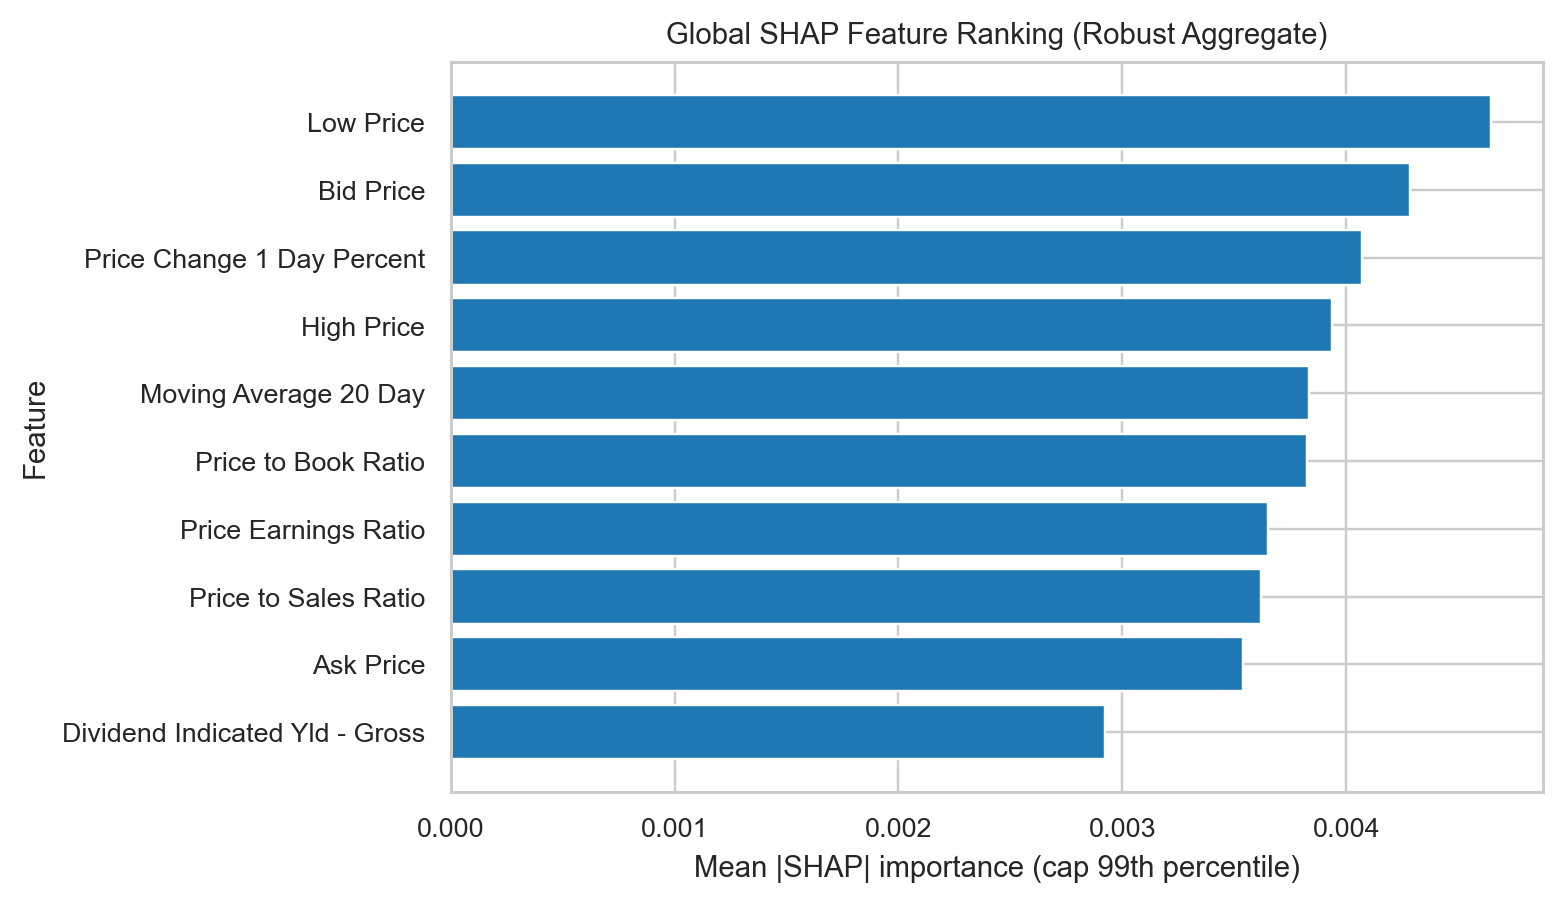
\includegraphics[width=\columnwidth]{images/shap_global_ranking_bar.png}
\caption{Global SHAP ranking using robust mean importance (99th-percentile capped).}
\label{fig:shap_global_bar}
\end{figure}

\begin{figure}[t]
\centering
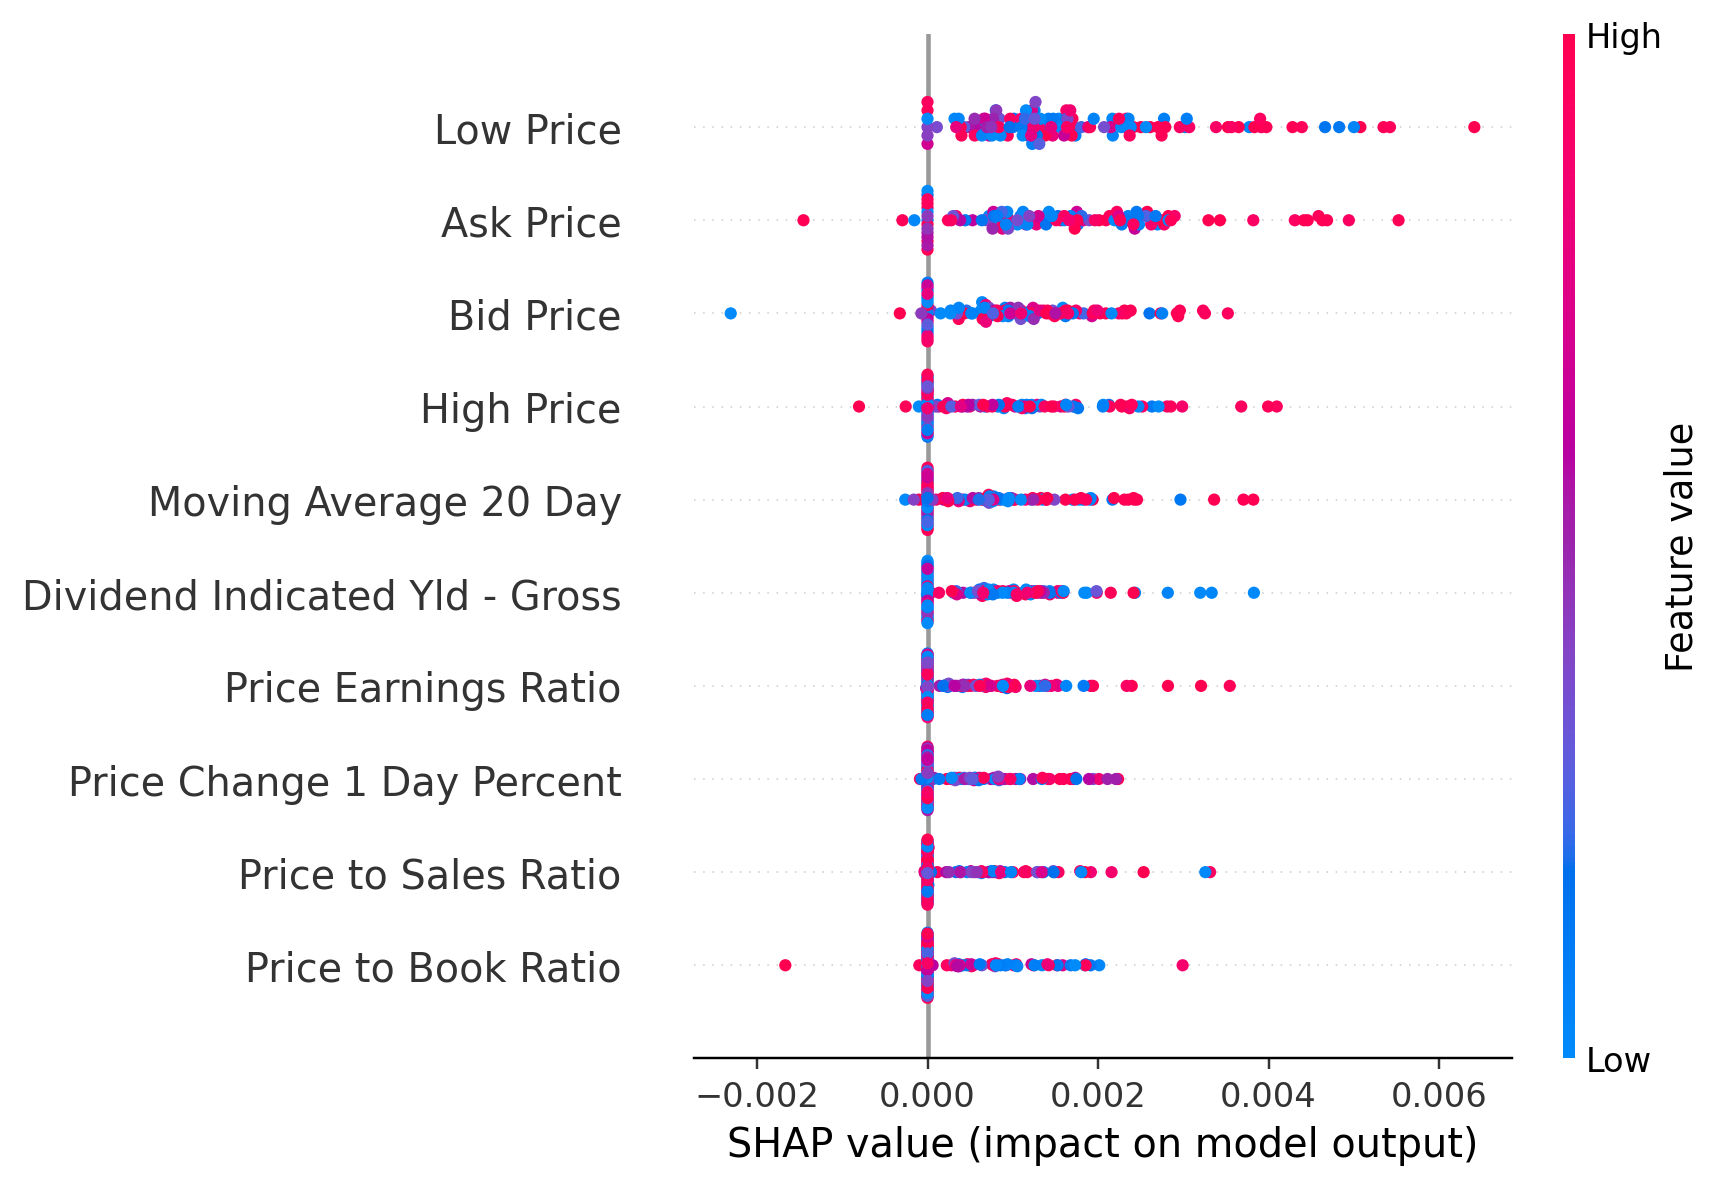
\includegraphics[width=\columnwidth]{images/shap_beeswarm_style_best.png}
\caption{SHAP beeswarm plot for the best-performing checkpoint (BBTN, BiLSTM\_Data\_GA, seed 62).}
\label{fig:shap_beeswarm_runs}
\end{figure}

\subsection{Discussion and Threats to Validity}
Three validity points are important. First, the chronological split is fixed; different split boundaries may change relative ranking. Second, seed-level Wilcoxon tests are underpowered with $n=5$, which explains why several improvements with very small DM $p$-values are not mirrored by Wilcoxon significance. Third, optimization benefits are heterogeneous across banks, indicating risk of overfitting when tuning is not controlled.

Future work will extend this benchmark through walk-forward validation, larger seed counts, and broader stress-testing across additional market regimes for stronger temporal robustness.
